\subsection{Further Insights}

\subsubsection{Experimental Procedure}

In this experiment, we aimed to empirically investigate further the
characteristics of {\model} in reflecting the semantic accuracy in
migrated results. To achieve that, we focused on the migrated code
that {\model} works well, \ie {\model} scores reflect well the
semantic accuracy with respect to the reference code. Therefore, we
aimed to collect the set of migrated results whose {\model} scores
correlate highest to the semantic scores given by the human subject.

%Correlation coefficients are used in statistics to measure how strong
%a relationship is between two variable space. Concretely, in this case
%those variable space are semantic scores and {\model} scores.
%
%We aim to figure out specifics of a dataset in which {\model} can work
%well. Because {\model} was created to estimate the semantic of code
%translation, the dataset in which {\model} works well also is the
%dataset containing the high correlation between Semantic score and
%{\model}.

%\subsubsection{The Use of RANSAC}

To do that, we used an algorithm called Random Sample Consensus
(RANSAC)~\cite{Fischler:1981:RSC:358669.358692}. Given two spaces
({\model} scores and semantic scores) for a dataset of 375 pairs of
methods, RANSAC will return two sets: 1) a set of pairs called {\bf
  GOOD\_SET} containing the largest number of pairs and having highest
correlation coefficient between {\model} scores and semantic scores;
and 2) the complementary set of {\bf GOOD\_SET}, called {\bf
  BAD\_SET}, containing pairs with the scores inconsistent between two
spaces. Technically, RANSAC estimates a global relation that fits the
data, while simultaneously classifying the dataset into an inlier set
including the data points consistent with the relation and an outlier
set including points not consistent with the relation. More details
can found in~\cite{Fischler:1981:RSC:358669.358692}.

%RANSAC is a simple, yet powerful, technique that is commonly applied
%to the task of estimating the parameters of a model, using data that
%may be contaminated by outliers. 
%
%RANSAC estimates a global relation that fits the data, while
%simultaneously classifying the data into a inlier set including points
%consistent with the relation and a outlier set including points not
%consistent with the relation.

%In our research scope, we use RANSAC as a mean of data classifier
%which returns a set of pairs called \textbf{GOOD\_SET} contributing to
%the correlation between {\model} and semantic score and another set of
%pairs called \textbf{BAD\_SET} inconsistent the correlation.

%Due to its ability to tolerate a large fraction of outliers, the algorithm is a popular choice for a variety of robust estimation problems.


%RANSAC assumes that the training data consists of inliers that can be explained with the model and outliers that are gross-erroneous samples which do not fit the model at all. So using outliers when training the model would increase our final prediction error, as they contain almost no information about the model. 



%\subsubsection{Experiments}
Since RANSAC is a learning algorithm, we conducted independtly 10
experiments with RANCSAC running on the same dataset of translated
code from the model \textbf{mppSMT}. The data set contains 375 method
pairs representing {\model} and Semantic score caculated for the set
of traslated methods of
\textbf{mppSMT}. Table~\ref{table:RANSAC_experiments} shows the
results of our 10 times, which contains the number of pairs in
\textbf{GOOD\_SET} and the correlation coefficient corresponding to
each subset for each time.
%
The size of each subset ranges from 224 to 315, while the their
correlation value is at high rate (between 0.93 and 0.95).  From the
table, we chose the subset with the \textbf{median} of the correlation
values as \textbf{GOOD\_SET}. That is the experiment number 5
(correlation = 0.954874293) in the table and the number of pairs is
308.

%Figure~\ref{fig:inliers_outliers} shows the result of experiment No5 gained from RANCSAC.

\begin{table}
	\caption{RANSAC experiments}
	\begin{tabular}{|c|c|c|c|c|}
		\hline
		Experiment Number & Number of pairs & Correlations of inliers \\
		\hline
		10	& 315	& 0.934700727 \\		
		8	& 312	& 0.945424846 \\	
		9	& 312	& 0.947983773 \\
		4	& 310	& 0.948196013 \\
		{\cellcolor[gray]{.8}}5	& {\cellcolor[gray]{.8}}308	& {\cellcolor[gray]{.8}}0.954874293 \\
		7	& 244	& 0.955112418 \\	
		1	& 283	& 0.957661146 \\
		3	& 303	& 0.958122675 \\
		2	& 298	& 0.958659967 \\
		6	& 277	& 0.959811603 \\		
		\hline
	\end{tabular}
	\label{table:RANSAC_experiments}
\end{table}

%\begin{figure}[t]
%	\caption{An example: Dataset in experiment No5 classified into inlier points(green) and outlier point(yellow)}
%	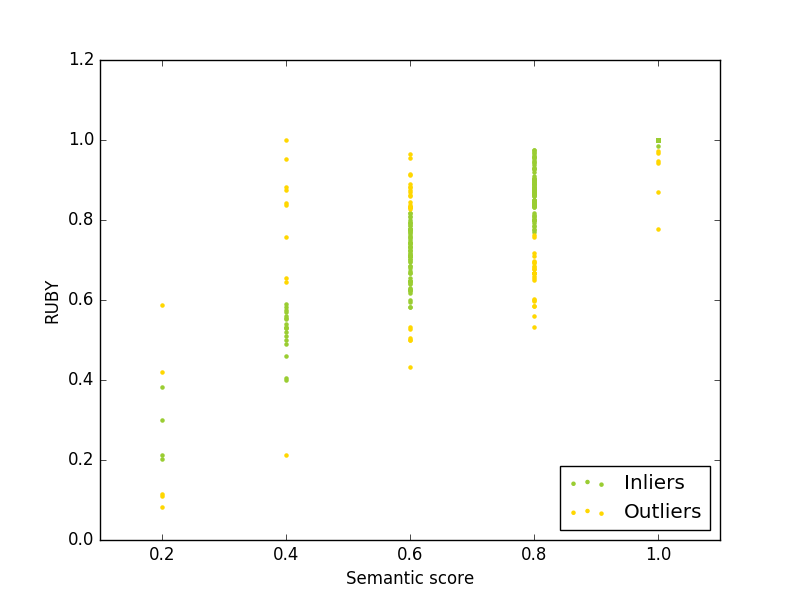
\includegraphics[scale=0.4]{img/inliers_outliers.png}
%	\centering
%	\label{fig:inliers_outliers}
%\end{figure}

\subsubsection{Result Categorization}

Examining \textbf{GOOD\_SET}, we classify each migrated result into
different groups with common characteristics. Our goal of
classification is to find the characteristics of {\model} to see how
it reflects correctly the semantic accuracy. For the {\bf BAD\_SET},
we also have the goal of understanding in which cases, {\model} does
not work well.

%the pairs of these sets into different groups that have common
%characteristics.  The principle for classification is that we aim to
%understand in which phenomenon {\model} could work well and could not
%work properly from \textbf{GOOD\_SET} and \textbf{BAD\_SET},
%respectively.


\textbf{GOOD\_SET.} {\model} works well on this dataset due to capturing certain features of code in lexical and structure terms as the groups descirbed below:

\begin{compactitem}
\item {\bf Group 1}: The translated code contains program elements with different lexical but same functionality with the reference. In this case, {\model} can capture these elements by using data dependency graph. For example, as can be seen in fig.~\ref{fig:mppSMT_example}, code translated by mppSMT used loop \textbf{for} which is the same meaning with \textbf{foreach} in the reference version. Besides, accessing to an array element could be implemented by  different ways such as \textbf{part[k]} or using iterator. The case number for this phenomenon is \textbf{32} over \textbf{308} pairs of the set.

\item {\bf Group 2}: Translated code contains the main program elements such as API names, method calls, variables reflected on the reference. even their usages are incorrect. By comparing tree representations - TRS, {\model} can capture these elements based on the common subtrees of translated and reference code. In the function \textbf{TestParserGrammarThere} of Fig.~\ref{fig:samples}, variable \textbf{grammar}, \textbf{found} and method call \textbf{Assert.AreEqual} appear in both translated and reference version but value assignments are not incorrect. There are \textbf{66} pairs involved in this situation.

\item {\bf Group 3}: Translated code contains the same structure and data flow with the reference. As can be seen from function \textbf{ContentAppend} Fig.~\ref{fig:samples}, the code structure in the translated version is similar to the reference with condition branches \textbf{if} and throwing exception \textbf{IllegalPdfSyntaxException}. {\model} can reflect semantic similarity by comparing code structure. By using GRS, {\model} can reflect similarity of source code in term of structure. Usually, when manually evaluate translation quality, developers have high regard for code structure. That is the reason for why {\model} can evaluate sematic well in this case. There is a majority of pairs falling into this group,  \textbf{112} pairs in total of \textbf{GOOD\_SET}, to be exact.
\end{compactitem}



\begin{figure}[t]
	\centering
	%\begin{lstlisting}[basicstyle=\small\sffamily, stepnumber=1, numbers=left, language=Java, aboveskip=1pt,  belowskip=1pt, numbersep=-5pt]
	\lstinputlisting[basicstyle=\scriptsize\sffamily,language=Java]{samples.cs}
	%\end{lstlisting}
	\caption{Sample}
	\label{fig:samples}
\end{figure}

\textbf{BAD\_SET.} The past Stephen Hawking said: "One of the basic rules of the universe is that nothing is perfect. Perfection simply does not exist". Although {\model} can detect and capture well in some cases listed above, {\model} still has some drawbacks. By analyzing method pairs from \textbf{BAD\_SET}, it can be seen that {\model} does not work well on incomplete code. It means that when it comes with the code having syntax errors, the RUBY's eveluation is not high accuracy. The reason is that when the code can not be compiled due to syntax errors, both PDGs and ASTs are not applicable and RUBY is built based on lexical. Measuring semantic using lexical has limits as mentioned in this work before like using BLEU. 


%\begin{table}[]
%	\centering
%	\caption{Inlier classification}
%	\label{table:inliers_result}
%	\begin{tabular}{|m{1cm}|m{3cm}|m{4cm}}
%		\hline
%		Type      & Category         & Description                                                                                                                    
%		\\
%		\hline
%		High behavior & IDENTIDFIED           & Code is the same with the reference                                                                                             \\
%		& SAME\_FUNC\_DIFF\_LEX & Code uses a variety expression for the same functionarity with the reference, e.g for vs foreach, array[i] vs array.get(i)\\
%		& SAME\_DATA\_FLOW      & Code has the same data flow with the reference but there are still incorrect pieces of code                                     \\
%		\hline
%		Low behavior  & SAME\_KEYWORDS        & Code has the same keywords with the reference, i.e API names, method calls, variables. However, their usage is incorrect           \\
%		& DISORDERED            & Code has some same pieces of code with the reference. However they are disordered                                               \\
%		& DIFFERENT             & Code is totally different from the reference \\
%		\hline                                                                                   
%	\end{tabular}
%\end{table}
%
%
%\begin{table}[]
%	\centering
%	\caption{Outlier classification}
%	\label{table:outliers_result}
%	\begin{tabular}{|m{1cm}|m{3cm}|m{4cm}}
%		\hline
%		Type      & Category         & Description                                                                                                                    
%		\\
%		\hline
%		High behavior &     INCOMPLETED       &  Code has a lot of syntax errors and it is not completed however it still has a majority of same piece with the reference which include unimportant information \\                                   
%		\hline
%		Low behavior  & ALGORITHM\_VARIETY        & Code has the same functionarity with the reference, however it has been implemented by other algorithm, the lexical and data flow is almost different           \\
%		\hline                                                                                   
%	\end{tabular}
%\end{table}
